\subsection{Computing Distributed Systems}\label{sec:distributed}
In this section we will introduce the distributed systems, which we are going to use. These systems will help us distribute the data across multiple machines, as well as perform distributed parallel computations. 

\subsubsection{Hadoop Distributed Filesystem}\label{sec:hadoopfilesystem}
HDFS is a technology of which the main goal is to increase fault tolerance on very large data systems. It is designed to be distributed across inexpensive commodity hardware, where recovery is done quickly and automatically. HDFS is run on a master-worker architecture where the \emph{master} node, maintain the namespace hierachy as well as the location of file blocks, this machine is called a \emph{namenode}. As shown in \Cref{fig:hadoop}, the namenode can be seen as the root of a HDFS cluster. \emph{Datanotes} take commands from the \emph{namenode}, such as deleting or replicating file blocks.

\begin{figure}[!htb]
  \centering
  \scalebox{0.75}{
    \begin{tikzpicture}[->,>=stealth',bend angle=45,auto]
      % Disks
      \node[cylinder,draw=black,thick,aspect=0.3,minimum height=1.3cm,minimum width=1cm,shape border rotate=90,cylinder uses custom fill,xshift=-5cm] (D1) {Disk};
      \node[cylinder,draw=black,thick,aspect=0.3,minimum height=1.3cm,minimum width=1cm,shape border rotate=90,cylinder uses custom fill,xshift=-2cm] (D2) {Disk};
      \node[cylinder,draw=black,thick,aspect=0.3,minimum height=1.3cm,minimum width=1cm,shape border rotate=90,cylinder uses custom fill,xshift=2cm] (D3) {Disk};
      \node[cylinder,draw=black,thick,aspect=0.3,minimum height=1.3cm,minimum width=1cm,shape border rotate=90,cylinder uses custom fill,xshift=5cm] (D4)  {Disk};
      \node[cylinder,draw=black,thick,aspect=0.3,minimum height=1.3cm,minimum width=1cm,shape border rotate=90,cylinder uses custom fill,xshift=5cm,yshift=5cm] (D5) {Disk};
      \node[cylinder,draw=black,thick,aspect=0.3,minimum height=1.3cm,minimum width=1cm,shape border rotate=90,cylinder uses custom fill,xshift=-5cm,yshift=5cm] (D6) {Disk};

      % Data nodes
      \path node at (0,0) [draw,shape=rectangle, style=rounded corners, minimum width=2cm, minimum height=2.5cm,xshift=-5cm,yshift=0.3cm,label={[yshift=-0.65cm]Data node}] (DN1) {};
      \path node at (0,0) [draw,shape=rectangle, style=rounded corners, minimum width=2cm, minimum height=2.5cm,xshift=-2cm,yshift=0.3cm,label={[yshift=-0.65cm]Data node}] (DN2) {};
      \path node at (0,0) [draw,shape=rectangle, style=rounded corners, minimum width=2cm, minimum height=2.5cm,xshift=2cm,yshift=0.3cm,label={[yshift=-0.65cm]Data node}] (DN3) {};
      \path node at (0,0) [draw,shape=rectangle, style=rounded corners, minimum width=2cm, minimum height=2.5cm,xshift=5cm,yshift=0.3cm,label={[yshift=-0.65cm]Data node}] (DN4) {};
      \path node at (0,0) [draw,shape=rectangle, style=rounded corners, minimum width=2cm, minimum height=2.5cm,xshift=-5cm,yshift=5.3cm,label={[yshift=-0.65cm]Data node}] (DN5) {};
      \path node at (0,0) [draw,shape=rectangle, style=rounded corners, minimum width=2cm, minimum height=2.5cm,xshift=5cm,yshift=5.3cm,label={[yshift=-0.65cm]Data node}] (DN6) {};

      % Namenodes
      \path node at (0,0) [draw,shape=rectangle, style=rounded corners, minimum width=2cm, minimum height=2.5cm,xshift=-2cm,yshift=5.3cm,label={[yshift=-0.65cm]Namenode}] (NN1) {};
      \path node at (0,0) [draw,shape=rectangle, style=rounded corners, minimum width=2cm, minimum height=2.5cm,xshift=2cm,yshift=5.3cm,label={[yshift=-0.65cm]Namenode}] (NN2) {};

      % Server
      \path node at (0,0) [draw,shape=rectangle, style=rounded corners, minimum width=2.5cm, minimum height=3.5cm,xshift=-5cm,yshift=0.6cm,label={[yshift=-0.65cm]Server}] (S1) {};
      \path node at (0,0) [draw,shape=rectangle, style=rounded corners, minimum width=2.5cm, minimum height=3.5cm,xshift=-2cm,yshift=0.6cm,label={[yshift=-0.65cm,xshift=-0.5cm]Server}] (S2) {};
      \path node at (0,0) [draw,shape=rectangle, style=rounded corners, minimum width=2.5cm, minimum height=3.5cm,xshift=5cm,yshift=0.6cm,label={[yshift=-0.65cm]Server}] (S3) {};
      \path node at (0,0) [draw,shape=rectangle, style=rounded corners, minimum width=2.5cm, minimum height=3.5cm,xshift=2cm,yshift=0.6cm,label={[yshift=-0.65cm,xshift=0.5cm]Server}] (S4) {};
      \path node at (0,0) [draw,shape=rectangle, style=rounded corners, minimum width=5.5cm, minimum height=3.5cm,xshift=-3.5cm,yshift=5.6cm,label={[yshift=-0.65cm]Server}] (S5) {};
      \path node at (0,0) [draw,shape=rectangle, style=rounded corners, minimum width=5.5cm, minimum height=3.5cm,xshift=3.5cm,yshift=5.6cm,label={[yshift=-0.65cm]Server}] (S6) {};

      % Cluster
      \path node at (0,0) [draw,shape=rectangle, style=rounded corners, minimum width=6cm, minimum height=9.5cm,xshift=-3.5cm,yshift=3.4cm,label={[yshift=-0.65cm]HDFS Cluster}] (C1) {};
      \path node at (0,0) [draw,shape=rectangle, style=rounded corners, minimum width=6cm, minimum height=9.5cm,xshift=3.5cm,yshift=3.4cm,label={[yshift=-0.65cm]HDFS Cluster}] (C2) {};

      % Stuff
      \path node at (0,0) [draw,shape=rectangle, style=rounded corners, minimum width=1.5cm, minimum height=0.5cm,xshift=-2cm,yshift=9cm,label={[yshift=-0.5cm]Router}] (M1) {};
      \path node at (0,0) [draw,shape=rectangle, style=rounded corners, minimum width=1.5cm, minimum height=0.5cm,xshift=2cm,yshift=9cm,label={[yshift=-0.5cm]Router}] (M2) {};
      \path node at (0,0) [draw,shape=rectangle, style=rounded corners, minimum width=1.5cm, minimum height=0.5cm,xshift=0cm,yshift=10cm,label={[yshift=-0.5cm]Router}] (M3) {};

      % Arrows
      \path (M3) edge (M1)
            (M3) edge (M2)
            (M1) edge (M3)
            (M2) edge (M3)
            (M1) edge (NN1)
            (NN1) edge (M1)
            (M2) edge (NN2)
            (NN2) edge (M2)
            (NN1) edge (DN1)
            (DN1) edge (NN1)
            ([xshift=0.5cm]NN1.south) edge ([xshift=0.5cm]DN2.north)
            ([xshift=0.5cm]DN2.north) edge ([xshift=0.5cm]NN1.south)
            (NN1) edge (DN5)
            (DN5) edge (NN1)
            ([xshift=-0.5cm]NN2.south) edge ([xshift=-0.5cm]DN3.north)
            ([xshift=-0.5cm]DN3.north) edge ([xshift=-0.5cm]NN2.south)
            (NN2) edge (DN4)
            (DN4) edge (NN2)
            (NN2) edge (DN6)
            (DN6) edge (NN2);
          \end{tikzpicture}
      }
      \caption{Hadoop cluster overview}\label{fig:hadoop}
\end{figure} 

Ensuring file coherency in a distributed filesystem can be a very complicated, which is why Hadoop employs a simple \emph{write once, read many} model, where data can either be written as a new file, or appended to an existing file. Hadoop is commonly used for file sizes in the Giga- and Terabyte range. Hadoop \emph{blocks} are used in the same manner as regular blocks on the disk, however the size of these block are significantly larger, set to 64MB by default. Larger block size reduce the time spent seeking for data, increasing overall transfer rates of the disk. Other central benefits from blocks, are the ability to distribute files larger than any single disk in the cluster, as well as replicate blocks across multiple nodes. Typically a block will be replicated to three locations, where two are placed at the same rack, and the third exist elsewhere in the cluster. The main benefit of block replication is fault tolerance, however the cluster also benefit from better load managing and an overall transfer speed increase on files. Fault tolerance of the namenode is crucial, as the master-worker pattern introduces a single point of failure. Hadoop introduces two strategies for handling namenode failue: Either by writing a backup of the filesystem metadata to multiple filesystems, or by using a secondary namenode, that continuous copy the \emph{edit-log} of the filesystem and periodically merge it to its own filesystem image. However using the secondary alone presents a risk of loss, as the secondary can lag behind the primary. Commonly both techniques are used, to benefit both from low downtime and no risk of data loss.

The HDFS client write files by making requests on the namenode to create a file. If the namenode creates a new file record, the client may then write the file to datanodes. The splitting of data into blocks and placement of blocks on datanotes is managed by a \emph{FSDataOutputStream}, which is a stream given to the HDFS client. The client read files in much the same way as writing them, when a file read is requested, a \emph{FSDataInputStream} is returned to the client. This stream handles which blocks from which locations that should be read. Block replicas are sorted in terms of distance to the client, such that if a block exist on the client itself, this will always be the prioritised block.~\cite{hadoopIntro}.

\subsubsection{MapReduce}\label{sec:mapreduce_programming_model}
MapReduce is a programming model which was developed by J.\@ Dean et al.~\cite{DeanMapReduce}, and is designed to be used in the context of \emph{big data}. The model is useful in the context of processing large amounts of data, clustering as well as utilising parallelism. The main reason for the success of the MapReduce model, is because it is easy for the programmer to do parallel programming, and its low-cost, high-compute property, that support commodity hardware in a cluster configuration. MapReduce is also well-suited for handling data large enough to not fit into a single disk.

The user has to construct the MapReduce procedure, which is a computation with two steps, where: 
\begin{description}
\item[Map] works by taking a set of key-value pairs. These pairs are turned into a new set of \emph{intermediate} key-value pairs where the value is now in a list with one element. The intermediate data is now grouped by their key and passed to Reduce.
\item[Reduce] receives the intermediate data, then appends all the values, with the same keys, to a single list with the same key, which is returned as the result.
\end{description}
This can be seen in \Cref{fig:mapreduce}, where the input data will be split into smaller pieces and distributed across the workers which have been assigned to mapping. The mapping then splits the input data into sets of key-value pairs $\{k_1,v_1\}$, the sorting by $k_1$ is the step after the split. The next step is that the workers which have been assigned to reduce receives these results where each worker is assigned specific keys to receive. These key-value pairs are then turned into new sets of $\{k_1, [v_1,v_2,v_3,\dots,v_x]\}$, which is returned as the result.

% The user has to construct a \emph{map} and \emph{reduce} procedure. The two procedures are split into the following actions:
%\begin{description}
%\item[Map:] Takes an input key-value pair and produces an \emph{intermediate} set of key-value pairs representing the input. The MapReduce library then groups all the intermediate values by associated keys and pass them to the reduce function.     
%\item[Reduce:] This procedure takes an intermediate key and an iterable set of values for that key, it then reduces by merging these values into a single value result.
%\end{description}

\begin{figure}[!htb]
  \centering
    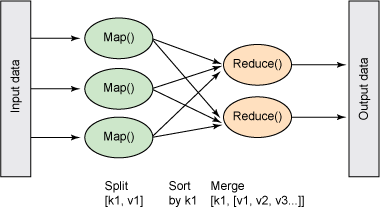
\includegraphics[width=0.50\textwidth]{img/mapreduceimage}
  \caption{The MapReduce Model}\label{fig:mapreduce}
\end{figure}

A common MapReduce example is the word count, in which a large document would be split into small fragments. These fragments would be sent to workers assigned to mapping, the mapping procedure would treat each individual word as a key and give it the value 1. This would give the intermediate result of $\{w_1,1\}, \{w_2,1\} \dots$. These intermediate results are then distributed across workers assigned to reduce such that all the pairs of e.g.\ $\{w_i,1\}$ are sent to the same worker. That worker appends the values with the same key, such that it becomes a key with a list of values, $\{w_i, [1,1,\dots] \}$. In this specific case an additional action is taken; the values of the list are summed up such that all the 1's are added together giving $\{w_i,1+1+\cdots \}$, which is then returned as result. The pseudo code for word count in MapReduce can be seen in \Cref{lst:mrwordcount}. 
\begin{lstlisting}[language=, caption={MapReduce Wordcount},label={lst:mrwordcount},belowcaptionskip=4pt]
map(name, document):
  for each word in document:
    emit (word, 1)

reduce(word, partialCounts):
  sum = 0
  for each partialCount in partialCounts:
    sum += partialCount
  emit (word, sum)
\end{lstlisting}
Here the map function take a document and its name as a key-value pair, and produce a new key-value pair for every word. The MapReduce Library groups values by the words and send the sets of $1s$ to the reducer function. The reducer then iterate through the value set, accumulating the amount of times that the word was found. Finally the reducer produces a single key-value pair, keeping the same key as its input.

\subsubsection{Apache Spark}\label{sec:spark}
Apache Spark is a general purpose cluster-computing system, that offers a high level programming API, as well as a set of high level tools for SQL data manipulation, machine learning and graph processing~\cite{sparkintro}. The main advantage of Spark compared to the MapReduce offered by Hadoop, is when working with iterative processes across the same data. Simply by keeping data cleverly in memory using Directed Acyclic Graphs, Spark performs iterative processes much faster. An example of a iterative task, is when computing the gradient for a logistic regression classification, the gradient for the separating hyperplane is found iteratively~\cite{ApacheSpark}.

A Spark application is a user application that is run by the a driver program, which handles the high level control flow of an application and distributes various operations across the cluster. Spark comprises of two important abstractions for distributed parallel computation: \emph{resilient distributed datasets}(RDD) and \emph{parallel operations} on these datasets. Furthermore, Spark also supports two types of shared variables that can be used in functions running on the cluster.

The RDD is a read-only collection of objects which is distributed across the machines in the cluster. RDDs are similar to a list structure when working with them. RDDs can live both in memory and on physical structure, and are fault-tolerant in the sense that they can be rebuilt because they contain information about how they were built. The parallel operations which are incorporated into Spark are: 
\begin{description}
  \item[Reduce:] Similar to the reduce action in MapReduce 
  \item[Collect:] All elements are sent to the driver program
  \item[Foreach:] Calls a function on each element in the RDD
\end{description}
\Cref{lst:wordcount} shows an example of a Spark application for counting words on a HDFS and output it into standard output.

\begin{lstlisting}[caption={Wordcount in Spark on HDFS},label={lst:wordcount},belowcaptionskip=4pt]
from pyspark import SparkContext
sc = SparkContext("spark://node1:7077")
text_file = sc.textFile("hdfs://node1:9000/dictionary.txt")
counts = text_file.flatMap(lambda line: line.split(" ")) \
                  .map(lambda word: (word, 1)) \
                  .reduceByKey(lambda a, b: a + b)
print counts.collect()
\end{lstlisting} 
The code can be run by invoking pyspark, which is similar to the python interpreter. When invoked, the application is submitted to Spark on \texttt{spark://node1:7077} through the sparkcontext. \texttt{text\_file} is an RDD with references to each line in the file on the HDFS. We then split each line on blank space, into arrays, which are flattened out by using flatmap. Each word is then sent a key-value pair and reduced by key, counting up the occurrences of the word. Lastly we use collect to print out words and their occurrences.




% \begin{figure}[!htb]
%   \centering
%   \scalebox{0.75}{
%     \begin{tikzpicture}[->,>=stealth',bend angle=45,auto]
%       % Tasks
%       \path node at (0,0) [draw,shape=rectangle, style=rounded corners, minimum width=1.5cm, minimum height=0.8cm,xshift=0cm,yshift=0cm,label={[yshift=-0.65cm]Task}] (T1) {};
%       \path node at (0,0) [draw,shape=rectangle, style=rounded corners, minimum width=1.5cm, minimum height=0.8cm,xshift=2cm,yshift=0cm,label={[yshift=-0.65cm]Task}] (T2) {};
%       \path node at (0,0) [draw,shape=rectangle, style=rounded corners, minimum width=1.5cm, minimum height=0.8cm,xshift=0cm,yshift=4cm,label={[yshift=-0.65cm]Task}] (T3) {};
%       \path node at (0,0) [draw,shape=rectangle, style=rounded corners, minimum width=1.5cm, minimum height=0.8cm,xshift=2cm,yshift=4cm,label={[yshift=-0.65cm]Task}] (T4) {};

%       % Caches
%       \path node at (0,0) [draw,shape=rectangle, style=rounded corners, minimum width=1.5cm, minimum height=0.8cm,xshift=2cm,yshift=1cm,label={[yshift=-0.65cm]Cache}] (C1) {};
%       \path node at (0,0) [draw,shape=rectangle, style=rounded corners, minimum width=1.5cm, minimum height=0.8cm,xshift=2cm,yshift=5cm,label={[yshift=-0.65cm]Cache}] (C2) {};

%       % Executor
%       \path node at (0,0) [draw,shape=rectangle, style=rounded corners, minimum width=3.75cm, minimum height=2.15cm,xshift=1cm,yshift=0.5cm,label={[yshift=-0.85cm,xshift=-1cm]Executor}] (E1) {};
%       \path node at (0,0) [draw,shape=rectangle, style=rounded corners, minimum width=3.75cm, minimum height=2.15cm,xshift=1cm,yshift=4.5cm,label={[yshift=-0.85cm,xshift=-1cm]Executor}] (E2) {};

%       % Worker
%       \path node at (0,0) [draw,shape=rectangle, style=rounded corners, minimum width=3.95cm, minimum height=3cm,xshift=1cm,yshift=0.75cm,label={[yshift=-0.55cm,xshift=-0.8cm]Worker node}] (W1) {};
%       \path node at (0,0) [draw,shape=rectangle, style=rounded corners, minimum width=3.95cm, minimum height=3cm,xshift=1cm,yshift=4.75cm,label={[yshift=-0.55cm,xshift=-0.8cm]Worker node}] (W2) {};

%       % Cluster Manager
%       \path node at (0,0) [draw,shape=rectangle, style=rounded corners, minimum width=3.5cm, minimum height=2cm,xshift=-4cm,yshift=2.75cm,label={[yshift=-1.25cm]Cluster manager}] (CM) {};

%       % SparkContent
%       \path node at (0,0) [draw,shape=rectangle, style=rounded corners, minimum width=3.25cm, minimum height=1cm,xshift=-9cm,yshift=2.5cm,label={[yshift=-0.80cm]SparkContent}] (SC) {};

%       % Driver Program
%       \path node at (0,0) [draw,shape=rectangle, style=rounded corners, minimum width=3.5cm, minimum height=2cm,xshift=-9cm,yshift=2.75cm,label={[yshift=-0.65cm]Driver Program}] (DP) {};

%       % Edges
%       \path ([xshift=1cm]E1.north) edge ([xshift=1cm]E2.south)
%       ([xshift=1cm]E2.south) edge ([xshift=1cm]E1.north)
%       (CM) edge (W1)
%       (CM) edge (W2)
%       (W1) edge (CM)
%       (W2) edge (CM)
%       (SC) edge ([yshift=-0.25cm]CM.west)
%       ([yshift=-0.25cm]CM.west) edge (SC)
%       (SC.south east) edge [bend right] (E1.west)
%       (E2.west) edge [bend right] (SC.north east)
%       (SC.north east) edge [bend left] (E2.west)
%       (E1.west) edge [bend left] (SC.south east);

%     \end{tikzpicture}
%   }
%   \caption{Spark setup overview}\label{fig:spark}
% \end{figure} 

%%% Local Variables:
%%% mode: latex
%%% TeX-master: "../main"
%%% End:
